% !TeX spellcheck = fr_FR
\title{%
	Mode d'emploi LoRa\\
	\large Un guide non exaustif de l'installation\\
	 compliquée d'une Gateway LoRa}
\date{27 avril 2023}
\author{Xavier Hueber\\Noé Lindelaub\\HE-ARC}
\fontsize{12}{12}
\documentclass{article}

%Margins
\usepackage{geometry}
\geometry{
	a4paper,
	left=19.1mm,
	right=19.1mm,
	top=25.4mm,
	bottom=25.4mm,
}

%Import packages
\usepackage{graphicx}
\usepackage{blindtext}
\usepackage[section]{placeins}
\usepackage{float}% If comment this, figure moves to Page 2
\usepackage{ragged2e}
\usepackage{framed}
\usepackage{mathtools} 
\usepackage{amsmath}
\usepackage{subcaption}
\usepackage{fancyhdr}
\usepackage[hidelinks]{hyperref}
\usepackage[citestyle=alphabetic,bibstyle=authortitle, backend=biber]{biblatex}
\bibliography{sources.bib}

\pagestyle{fancy}

\fancyhead{}
\fancyfoot{} % clear all footer fields
\fancyfoot[LO,CE]{Xavier Hueber \\ Noé Lindenlaub}
\fancyfoot[CO,RE]{\thepage}
\fancyfoot[LE,RO]{Mode d'emploi LoRa}

\justifying

%Custom Macros
\newcommand{\XHframebox}[1] 
{
	\noindent\framebox{\noindent
		\begin{minipage}{\dimexpr\linewidth-2\fboxrule-2\fboxsep\relax}
			#1
		\end{minipage}
	}
}
%Change table of contents name
\renewcommand{\contentsname}{Table des matières}
%Removes Bibliography from Table of contents

\begin{document}
	\maketitle
	\newpage
	\tableofcontents
	\newpage
	\section{Introduction}
		Ce guide créé dans le cadre du cours de Systèmes Communicants 2\textsuperscript\textcopyright, vous expliquera comment installer les logiciels nécessaires à la création d'une Gateway LoRa à partir d'un HAT Raspberry Pi Seeed disposant d'une puce RHF0M301.\\
		Nous utiliserons des nodes possédant d'un microprocesseur ESP32-S3 ainsi que d'un module série LoRa-E5-HF pour transmettre des messages par LoRaWAN\textsuperscript\textregistered.
		\subsection{Matériel utilisé}
			Dans le cadre de ce projet, nous avons utilisé:
			\begin{itemize}
				\item Un kit LoRa/LoRaWAN\textsuperscript\textregistered Gateway - 868MHz de Seeed.
				\item Un Raspberry Pi 3 modèle B.
				\item Deux ESP32-S3-DevKitC-1 v1.0 de Espressif.
				\item Deux modules LoRa-E5-HF de Seeed.
				\item Des antennes 868MHz SMA.
				\item Câble d'adaptation U-FL vers SMA.
				\item Une Gateway TheThingNetwork Kickstarter
				\item Une Gateway TheThingNetwork Indoor 
			\end{itemize}
		\subsection{Logiciels utilisés}
			Dans le cadre de ce projet, nous avons installé:
				\begin{itemize}
				\item Raspberry Pi OS 64-bit datant du 21 février 2023.
				\item Raspberry Pi Imager v1.7.4
				\item ChirpStack v3.
				\item RHF0M301-ChirpStack.
				\item Un éditeur de code moderne (ex: Sublime Text, VSCode, ...)
				\item Le compilateur IDF de Espressif
			\end{itemize}
		\subsection{Glossaire}
			\begin{center}
			\begin{tabular}{ ||c|c|| } 
				\hline
				Terme & Acronyme \\ [0.5ex]
				\hline \hline
				TheThingNetwork & TTN \\ 
				Carte d'extension du Raspberry Pi & HAT \\
				\hline
			\end{tabular}
			\end{center}
	\newpage
	\section{Installation}
		\subsection{Installation du Raspberry Pi}
			\subsubsection{Raspberry Pi OS}
				\XHframebox{Le Raspberry Pi nous servira à recevoir, gérer et retransmettre les paquets reçu par LoRaWAN\textsuperscript\textregistered.}
				
				Nous avons commencé par installer Rapsberry Pi OS 64 bit sur une carte sd grâce au logiciel Raspberry Pi Imager (voir figure \ref{fig:raspberrypiimager}).\\
				Dans celui-ci, nous pouvons activer la connexion SSH et configurer les logins de l'utilisateur, ainsi nous n'avons pas besoin d'utiliser un écran pour configurer le Raspberry Pi.
				\begin{figure}[H]
					\centering
					\begin{subfigure}{0.49\textwidth}
						\centering
						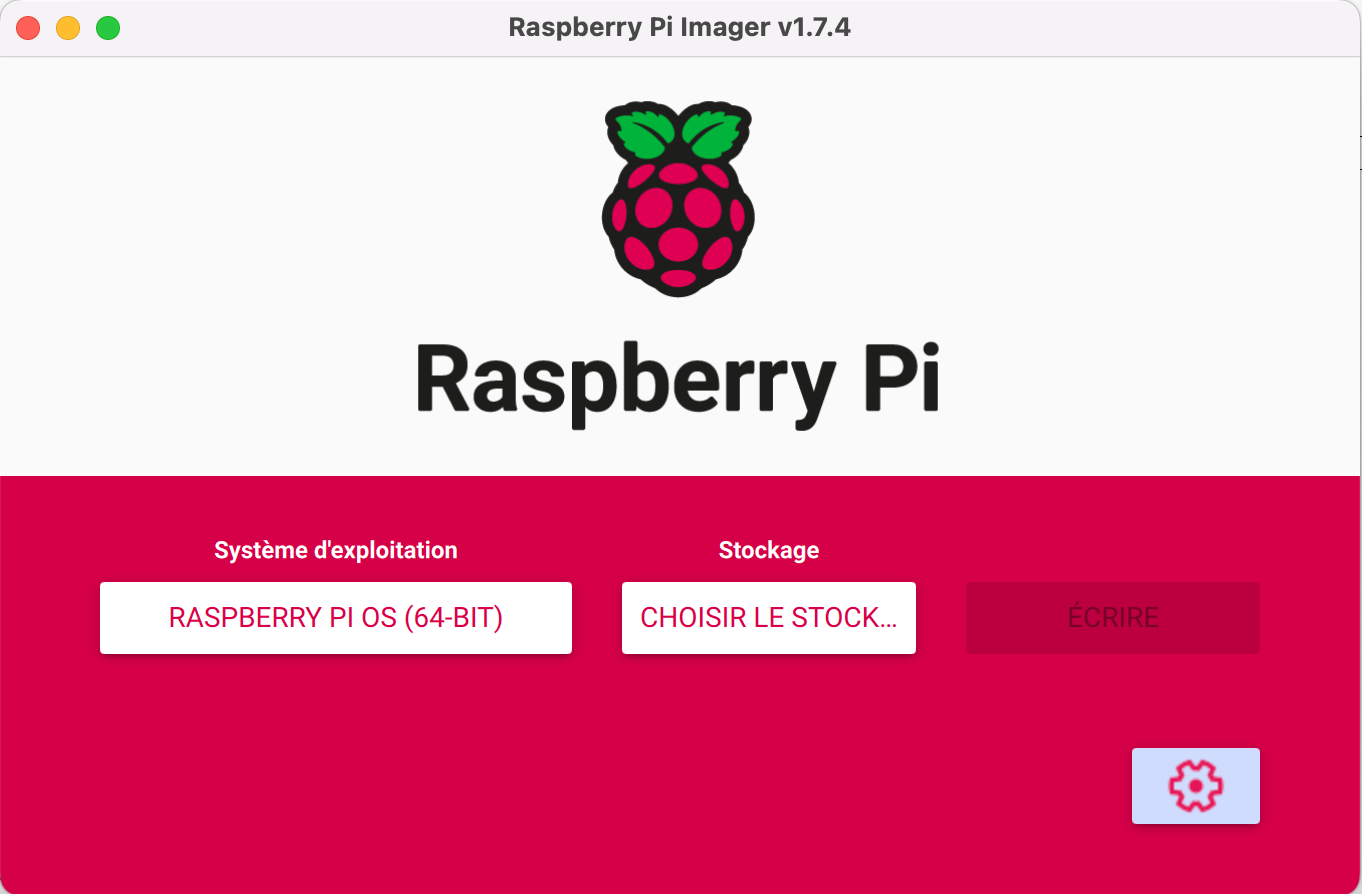
\includegraphics[width=\linewidth]{raspberrypi_imager}
						\caption{Menu}
						\label{fig:raspberrypiimager}
					\end{subfigure}
					\begin{subfigure}{0.49\textwidth}
						\centering
						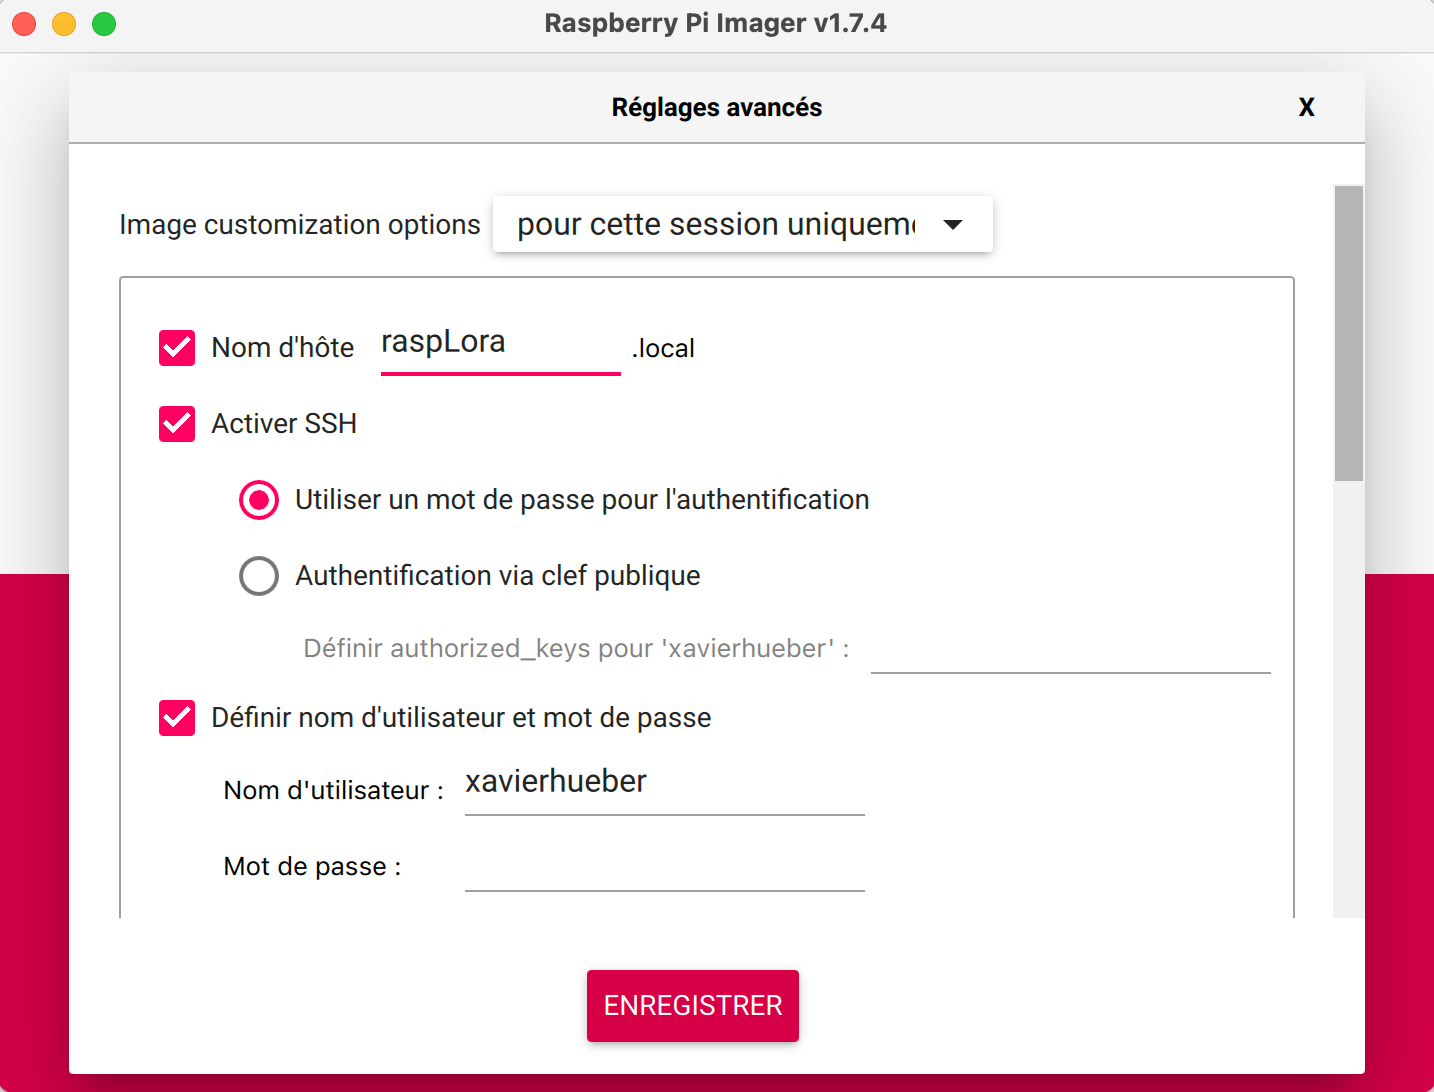
\includegraphics[width=\linewidth]{raspberrypi_imager1}
						\caption{Configuration du SSH et de l'utilisateur}
						\label{fig:raspberrypiimager1}
					\end{subfigure}
					\caption{Raspberry Pi Imager}
				\end{figure}
			\subsubsection{Logiciels tiers}
				Maintenant que nous avons installé un système d'exploitation sur le Raspberry Pi, nous pouvons installer une application pour récupérer et gérer les paquets LoRaWAN\textsuperscript\textregistered.
				
				Nous voulions pour cela installer l'application proposé par Seeed pour l'utilisation de leur HAT, cependant nous n'avons pas trouvé de liens de téléchargement ni de guide d'installation disponible sur leur site web. 
				Nous avons alors commencé par chercher des applications tierces compatible avec le module RHF0M301. Une solution simple était d'installer basicstation, un logiciel développé par TTN qui transfère tous les paquets vers leurs serveurs.
				
				Cependant, nous ne voulions pas pour commencer des tests, être dépendant de TTN et de leurs services (ceux-ci étant fortement limités à 30 secondes d'émission par jour).
				Nous avons alors décidé de chercher une autre solution et sommes tombés sur ChirpStack\footnote{\url{https://www.chirpstack.io/docs/chirpstack-gateway-bridge/install/raspberry-pi.html}}. ChirpStack est un ensemble d'applications permettant la réception, l'envoi et la gestion de paquets LoRaWAN\textsuperscript\textregistered comme basicstation, mais elles permettent de gagner en flexibilité car chaque étape de traitement des paquets sont fait par une autre application de façon totalement indépendante.
				
				\paragraph{ChirpStack nous donne ainsi accès au système que vous pouvez voir dans la figure \ref{fig:systemechirpstack}:}
				\begin{enumerate}
					\item L'application Gateway viens communiquer avec le HAT du Raspberry Pi 3 et publie les informations reçues par MQTT.
					\item Le Network Server récupère alors les informations et les traite pour qu'elles soient utilisable par la User Application et publie sur MQTT.
					\item La ou les User(s) Application(s) souscrivent au Network Server et reçoivent alors les informations traités.
				\end{enumerate}

				\begin{figure}[H]
					\centering
					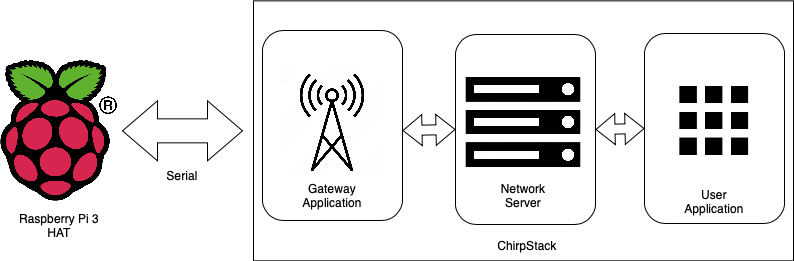
\includegraphics[width=0.7\linewidth]{Systeme_ChirpStack}
					\caption{Système applicatif ChirpStack}
					\label{fig:systemechirpstack}
				\end{figure}
				
		\subsection{Installation de l'environnement de développement Espressif}
			Maintenant que nous avons installé les tools requis pour faire fonctionner le Raspberry Pi, nous pouvons passer à l'installation de la toolchain ESP afin de pouvoir programmer nos deux Devkits. 
			\newline
			\newline
			Pour ce faire, nous nous rendons sur le site d'espressif et suivons le guide d'installation\footnote{\url{https://docs.espressif.com/projects/esp-idf/en/latest/esp32s3/get-started/index.html\#get-started-step-by-step}}. 
			\newline
			Nous avons ensuite compilé et flasher le projet Hello-World\footnote{Voir notre répertoire Github} pour tester le fonctionnement de la carte. C'est avec succès que celle-ci s'est mise en route et nous a donné ses premiers mots.
			
	\section{Programmation du Devkit ESP}
		Nous avons commencé par étudier la documentation fournie par Seeed pour son  module LoRa-E5-HF. Sachant qu'il se pilote par série, il nous a fallu comprendre comment utiliser le port série du Devkit ESP.
		
		Pour cela, nous avons trouvé l'exemple uart\_echo donné par Espressif qui nous a permis de comprendre comment configurer et utiliser l'uart.
		
		Nous avons ensuite importé un partie du code de uart\_echo dans notre application LoRa\_send et utilisé les commandes AT que nous avions testé à la mains auparavant. Voici quelques commandes AT disponibles intéressantes ainsi que leur utilité:
		\begin{center}
			\begin{tabular}{ ||c|c|| } 
				\hline
				Commande AT & Utilisation \\ [0.5ex]
				\hline \hline
				AT & Répond AT+ pour dire que tout se passe bien \\ 
				AT+UART=BR, {baudrate} & Permet de choisir le baudrate au prochain démarrage du module \\
				AT+KEY= APPKEY, "KEY" & Permet de configurer l'AppKey utilisé lors de l'envoi de paquets LoRa \\
				AT+MODE=LWOTAA & Permet de configurer le mode de connexion à la Gateway \\
				AT+JOIN & Permet de rejoindre la Gateway \\
				AT+MSG="CestNoe" & Permet d'envoyer un paquet LoRa contenant le message spécifié \\
				AT+CMSG="CestNoe" & Envoi un paquet et demande une confirmation \\
				AT+POWER=14 & Permet de choisir la puissance d'émission en dB \\
				\hline
			\end{tabular}
		\end{center}
		
		Comme vous pouvez le voir dans la figure \ref{fig:lorasend}, le programme est assez simple. Nous commençons par configurer la connexion UART requise pour communiquer avec le module LoRa, puis nous configurons ce dernier (voir figure \ref{fig:atlorasend}) et enfin nous avons écrit une boucle while qui envoi en boucle tous les X temps un message incrémenté.
		\begin{figure}[H]
			\centering
			\begin{subfigure}{0.20\textwidth}
				\centering
				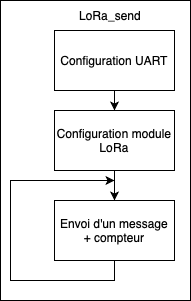
\includegraphics[height=15em]{LoRa_send.drawio}
				\caption{Diagramme du logiciel LoRa\_send}
				\label{fig:lorasend}
			\end{subfigure}
			\begin{subfigure}{0.70\textwidth}
				\centering
				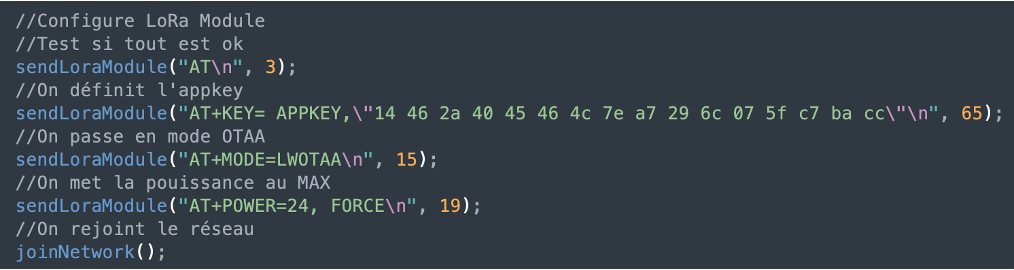
\includegraphics[width=1\linewidth]{atLorasend}
				\caption{Configuration du module LoRa}
				\label{fig:atlorasend}
			\end{subfigure}
			\caption{LoRa\_send}
		\end{figure}
	
	\section{Configuration de ChirpStack}
		Nous avions vu précédemment que nous avions installé ChirpStack sur notre Raspberry Pi, il est maintenant temps de configurer ce stack d'applications pour pouvoir recevoir nos paquets LoRa.
		La configuration n'est pas compliqué, mais il faut quand même suivre un ordre précis sinon vous ne pourriez vous retrouver coincé. Cette dernière se fera dans l'interface web de ChirpStack disponible sur le port 8080 du Raspberry Pi.
		
		\subsection{Network Server}
			Dans un premier temps il va falloir configurer le Network Server, c'est lui qui est gère les paquets. Dans la figure \ref{fig:networkserver} vous pouvez voir qu'on lui donne l'adresse localhost:8000 car ce dernier est installé en local. Si nous voulions mettre en place une plus grande architecture de Gateways, nous pourrions ainsi dédié un serveur unique comme étant le Network Server.
			\begin{figure}[H]
				\centering
				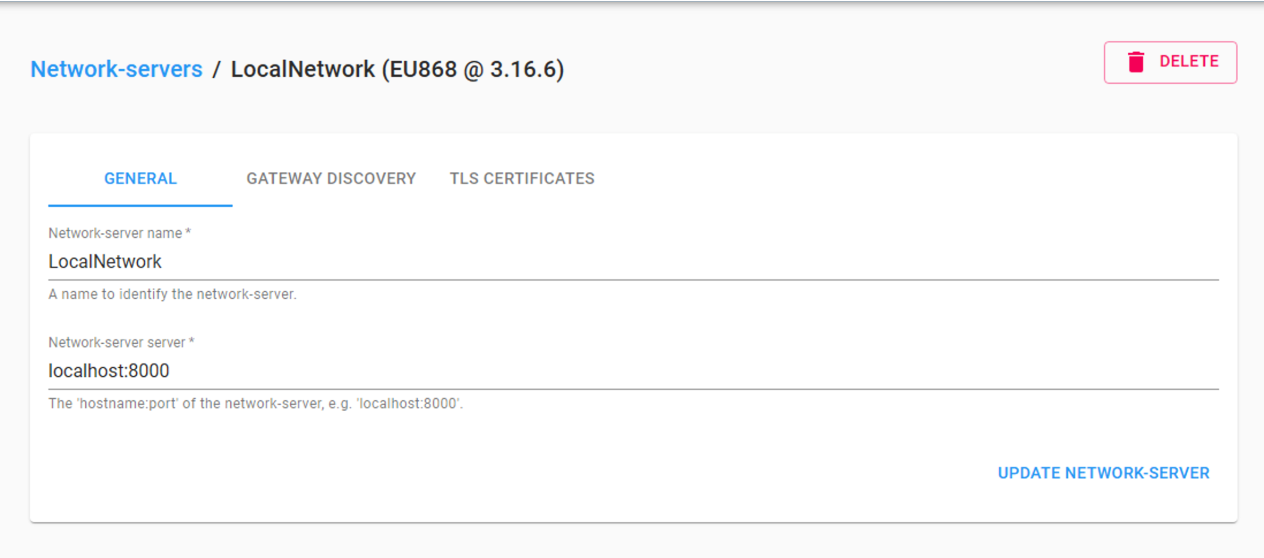
\includegraphics[width=0.7\linewidth]{networkserver}
				\caption{Network Server}
				\label{fig:networkserver}
			\end{figure}
		
		\subsection{Gateway Profile}
			Cette étape n'est pas une des plus intéressantes et cette option mériterait d'être configuré directement lors de la création de la Gateway dans l'interface de Chirpstack. Le profile de la Gateway permet de choisir le temps entre deux récupération de paquets du HAT Raspberry Pi.
			
			On peut voir sur la figure \ref{fig:gateway-profile} les options disponibles et comment nous les avons configurés. 
			
			\begin{figure}[H]
				\centering
				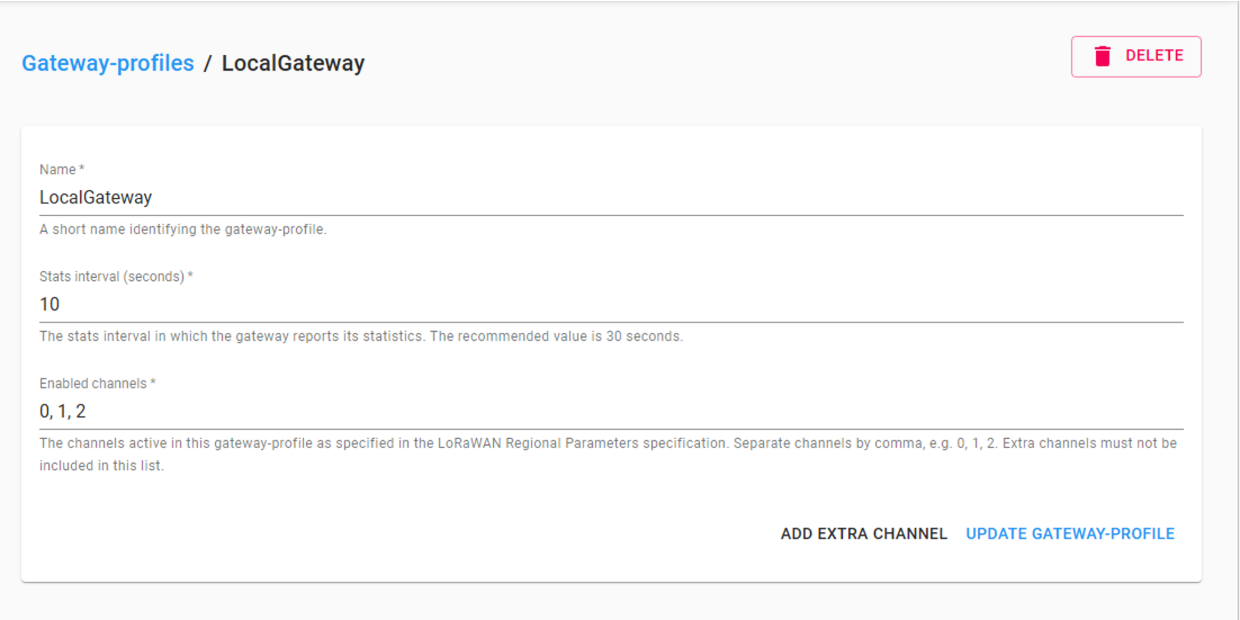
\includegraphics[width=0.7\linewidth]{gateway-profile}
				\caption{Gateway profiles}
				\label{fig:gateway-profile}
			\end{figure}
		
		\subsection{Device Profile}
			La configuration du Device profile permet de choisir comme son nom l'indique un profile pour les nodes LoRa que nous auront.
			On peut entre autre y choisir la version de LoRaWAN\textsuperscript\textregistered supporté ainsi que la classe de la node et le mode de connection à la Gateway.
			
			On peut voir sur la figure \ref{fig:device-profile} que nous utilisons la version 1.0.4 de LoRaWAN et pour le mode de connection nous utilisons le LWOTAA comme spécifié plus haut dans le programme LoRa\_send pour l'ESP32.
						
			\begin{figure}[H]
				\centering
				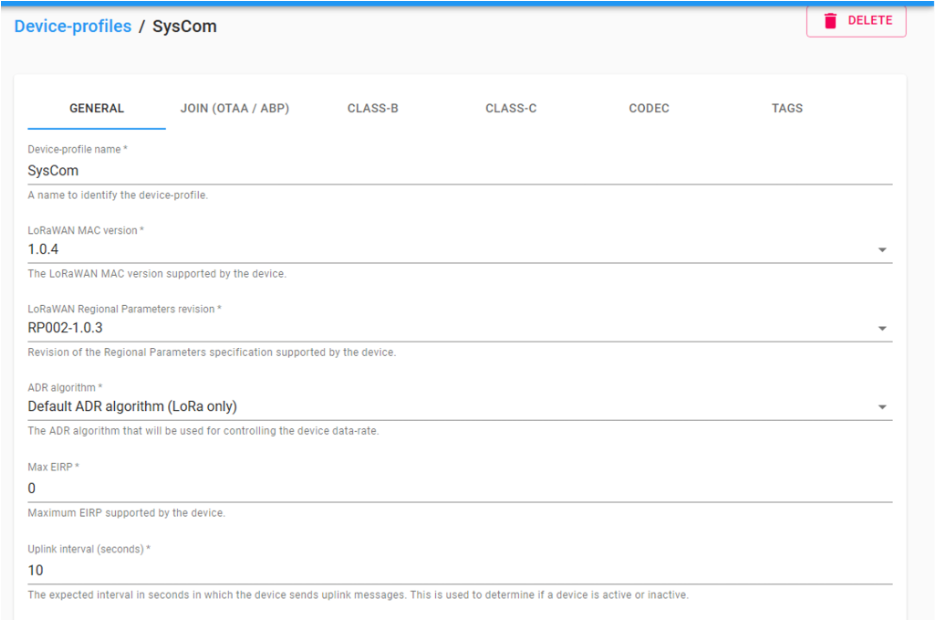
\includegraphics[width=0.7\linewidth]{device-profile}
				\caption{Device profile}
				\label{fig:device-profile}
			\end{figure}
			
		\subsection{Gateway}
			Nous pouvons maintenant configurer la Gateway:
			
			Dans ce menu (voir figure \ref{fig:gateway}), nous pouvons donner un nom à notre Gateway et un ID (généré aléatoirement en général). Il faut ensuite choisir le Network Server avec qui elle va communiquer et le Gateway profile.
			\begin{figure}[H]
				\centering
				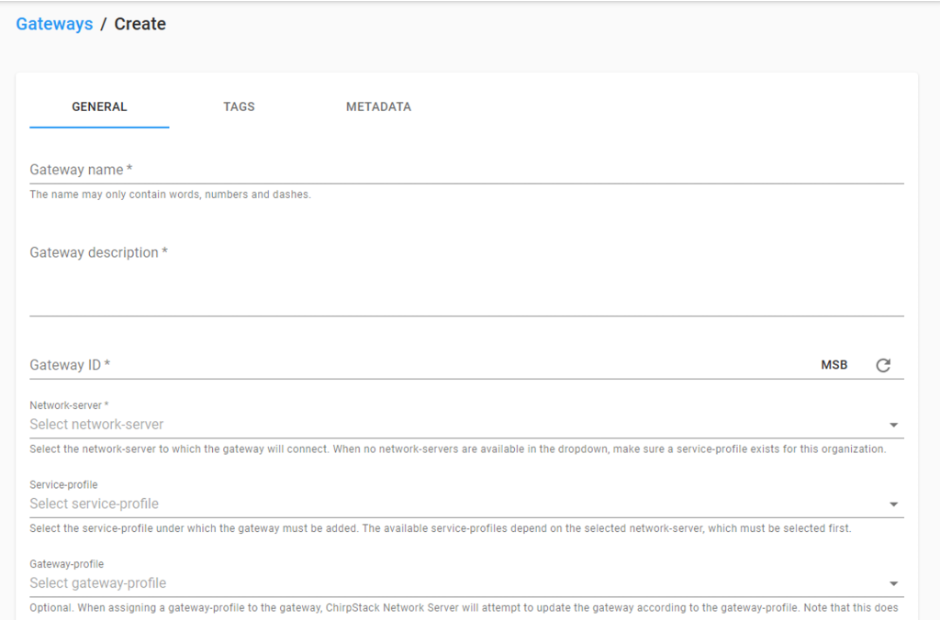
\includegraphics[width=0.7\linewidth]{gateway}
				\caption{Configuration de la Gateway}
				\label{fig:gateway}
			\end{figure}
			
		\subsection{Application}
			Une application est un groupement de nodes, une fois créé elle permettra d'ajouter des nodes qui pourront se connecter à notre Gateway et c'est aussi dans l'Application que nous pourront choisir comment seront envoyé les paquets vers internet (voir le Chapitre \ref{internet}).
			
			Dans la figure \ref{fig:application}, on peut donc choisir un nom pour notre Application et une description.
			
			\begin{figure}[H]
				\centering
				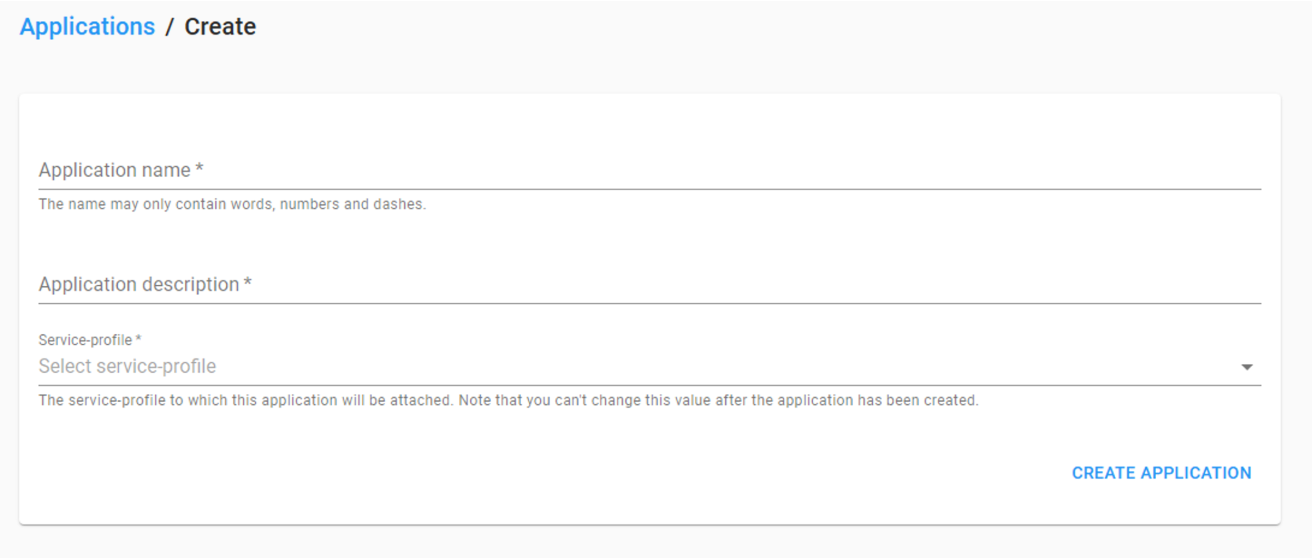
\includegraphics[width=0.7\linewidth]{application}
				\caption{Configuration d'une application}
				\label{fig:application}
			\end{figure}
			
		\subsection{Device}
			Enfin la dernière chose à configurer dans ChirpStack est la création d'une node.
			
			Dans le menu de l'application nous pouvons ajouter un nouveau device, vous verrez alors apparaitre la figure \ref{fig:device}.
			
			Ici il faut donc donner à un nom à notre node, un profil et un EUI qui correspond à l'identifiant de la node. Sur notre module LoRa Seeed, nous pouvons utiliser la commande série AT+ID=DevEui pour que le module nous donne son EUI.
			
			Ensuite une fois que ces informations sont remplis, on peut créer le device et ChirpStack nous proposera alors de générer une APPKEY. Cette dernière est très importante car elle est la clé permettant à la node de se connecter à la Gateway, sans elle la Gateway refusera la node. On peut ensuite copier l'APPKEY et la coller dans le programme LoRa\_send.
				
			\begin{figure}[H]
				\centering
				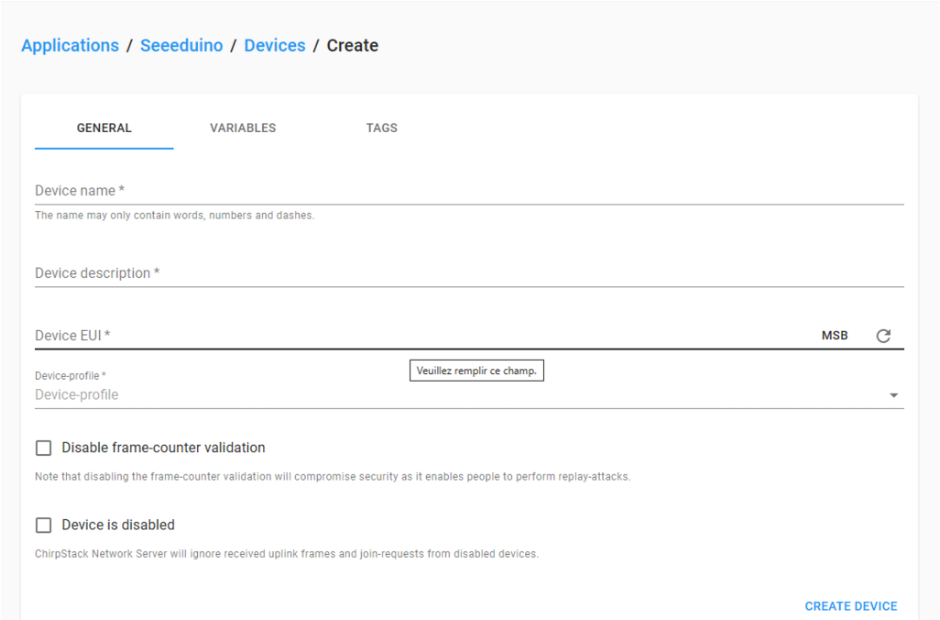
\includegraphics[width=0.7\linewidth]{device}
				\caption{Configuration d'une node}
				\label{fig:device}
			\end{figure}
			
			Si la node après ça n'arrive pas à se connecter à la Gateway, il faudra voir si les versions de LoRaWAN sont les mêmes entre celle donné dans le Device-Profile et celle configuré sur la node.
			
			On peut aussi utiliser le site LoRaWAN 1.0.x packet decoder\footnote{\url{https://lorawan-packet-decoder-0ta6puiniaut.runkit.sh}} pour voir si il y a un conflit d'APPKEY.
		
	\section{Envoi des paquets sur internet}
		\label{internet}
		\XHframebox{La node arrive maintenant à envoyer des paquets LoRaWAN à la Gateway, cependant dans l'interface de ChirpStack nous recevons les messages sous formes de JSON et la donnée est en base64.}
		
		Nous voulions alors pouvoir traiter ces messages pour ne récupérer que les informations les plus importantes.  ChirpStack nous permet alors d'utiliser d'autres applications comme MQTT ou Azure Service Bus (qui est une forme de MQTT propriétaire) pour envoyer les messages vers internet.
		
		Nous avons testés plusieurs services, mais celui qui a fonctionné pour le mieux est Azure Service Bus. Vous pouvez voir sur la figure \ref{fig:scriptpython} un diagramme montrant comme les messages sont envoyés et transformés à l'aide d'un script python\footnote{Vous pouvez retrouver ce script dans notre répertoire Github} vers Telegram.
		
		\begin{figure}[H]
			\centering
			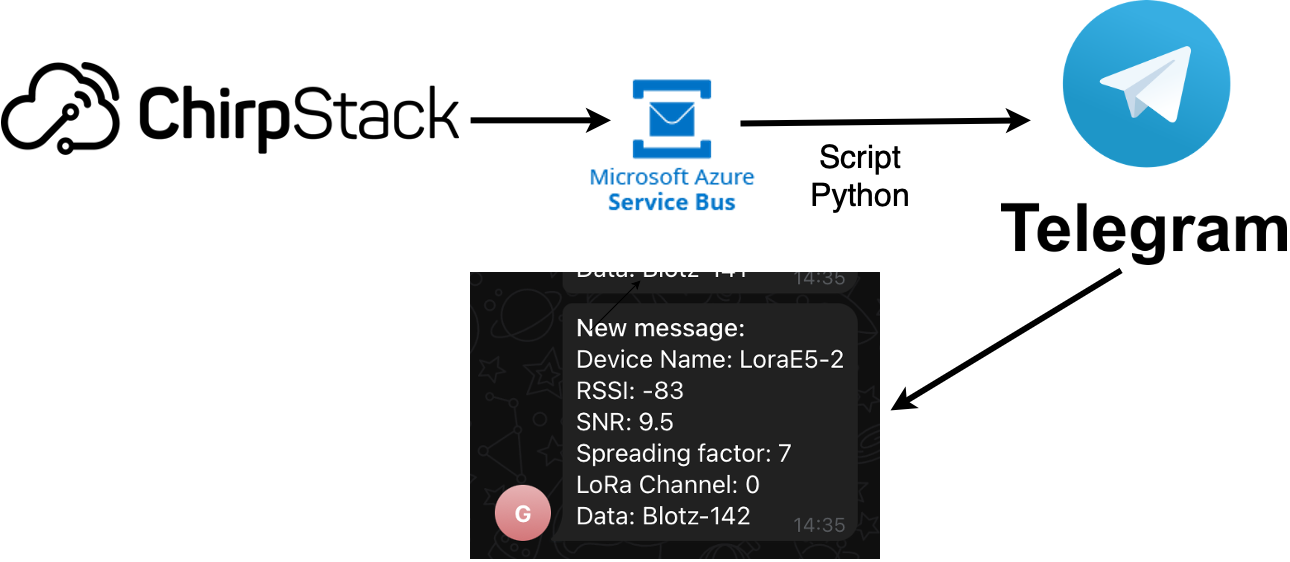
\includegraphics[width=0.7\linewidth]{scriptPython}
			\caption{Script python}
			\label{fig:scriptpython}
		\end{figure}
		
	\newpage
	\section{Version}
		\begin{itemize}
			\item Version 1.0 : 7 mai 2023 - Version originale
		\end{itemize}
\end{document}